\chapter{Planificación Inteligente}

Podemos ver la Planificación Inteligente desde varios puntos de vista:
\begin{itemize}
   \item Deducción\\
   A partir de algunos hechos ciertos, concer qué otros hechos también son ciertos (propagación)
   \item Aprendizaje\\
   ``Mejorar la conudcta a partir de la experiencia''
   \item Razonamiento sobre acciones
   A partir de lagunos hechos ciertos (estado inicial), decidir qué acciones se deben ejecutar para alcanzar ciertos objectivos (es decir, que otros hechos sean también ciertos) en base a relaciones de causa-efecto. 
\end{itemize}

El ser humano es inteligente porque es capaz de razonar acerca de las consecuencias de sus actos. Al fin y al cabo estamos planificando constantemente aunque no nos demos cuenta.

\begin{figure}[htbp]
   \centering
   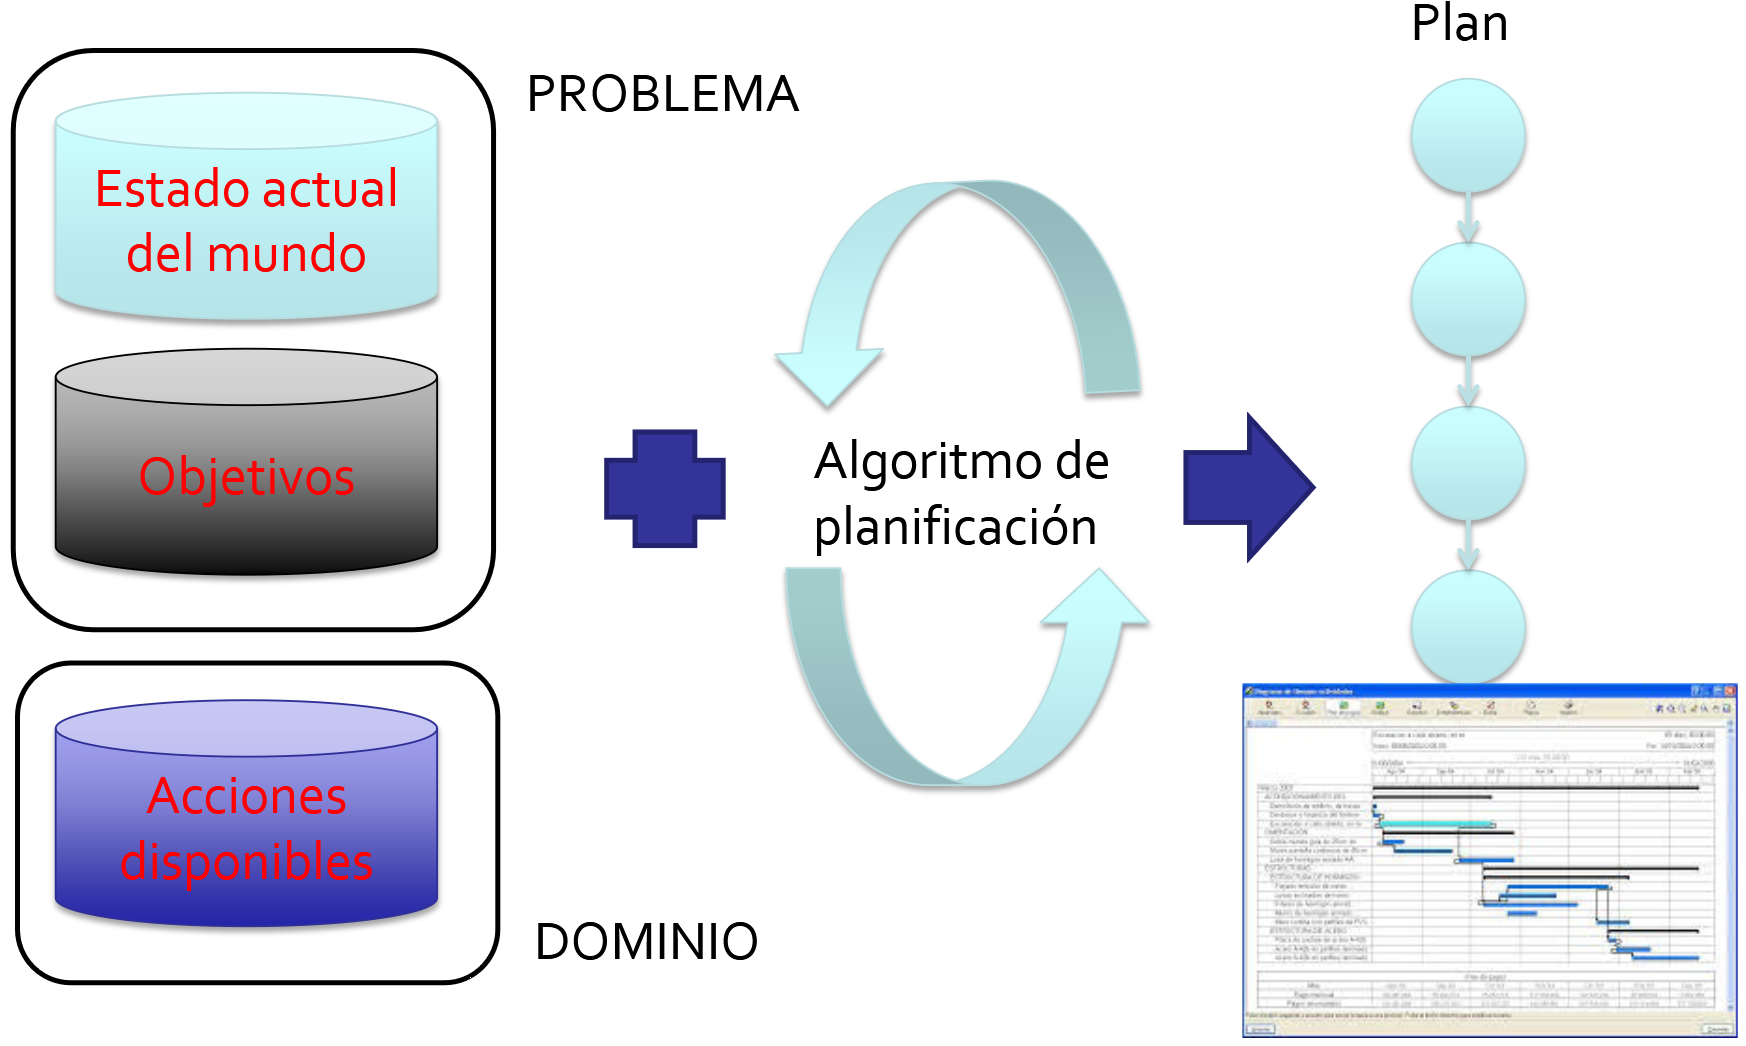
\includegraphics{images/02/planificacion.png}
   \caption{Planificación esquematizada}
   \label{fig:02/planificacion}
\end{figure}

En Fig. \ref{fig:02/planificacion} podemos ver un esquema de planificación. En el estado actual del mundo corresponde al \textit{``\textbf{dominio}''}, y el objetivo es llegar a un estado deseado nel mundo.

\begin{figure}[htbp]
   \centering
   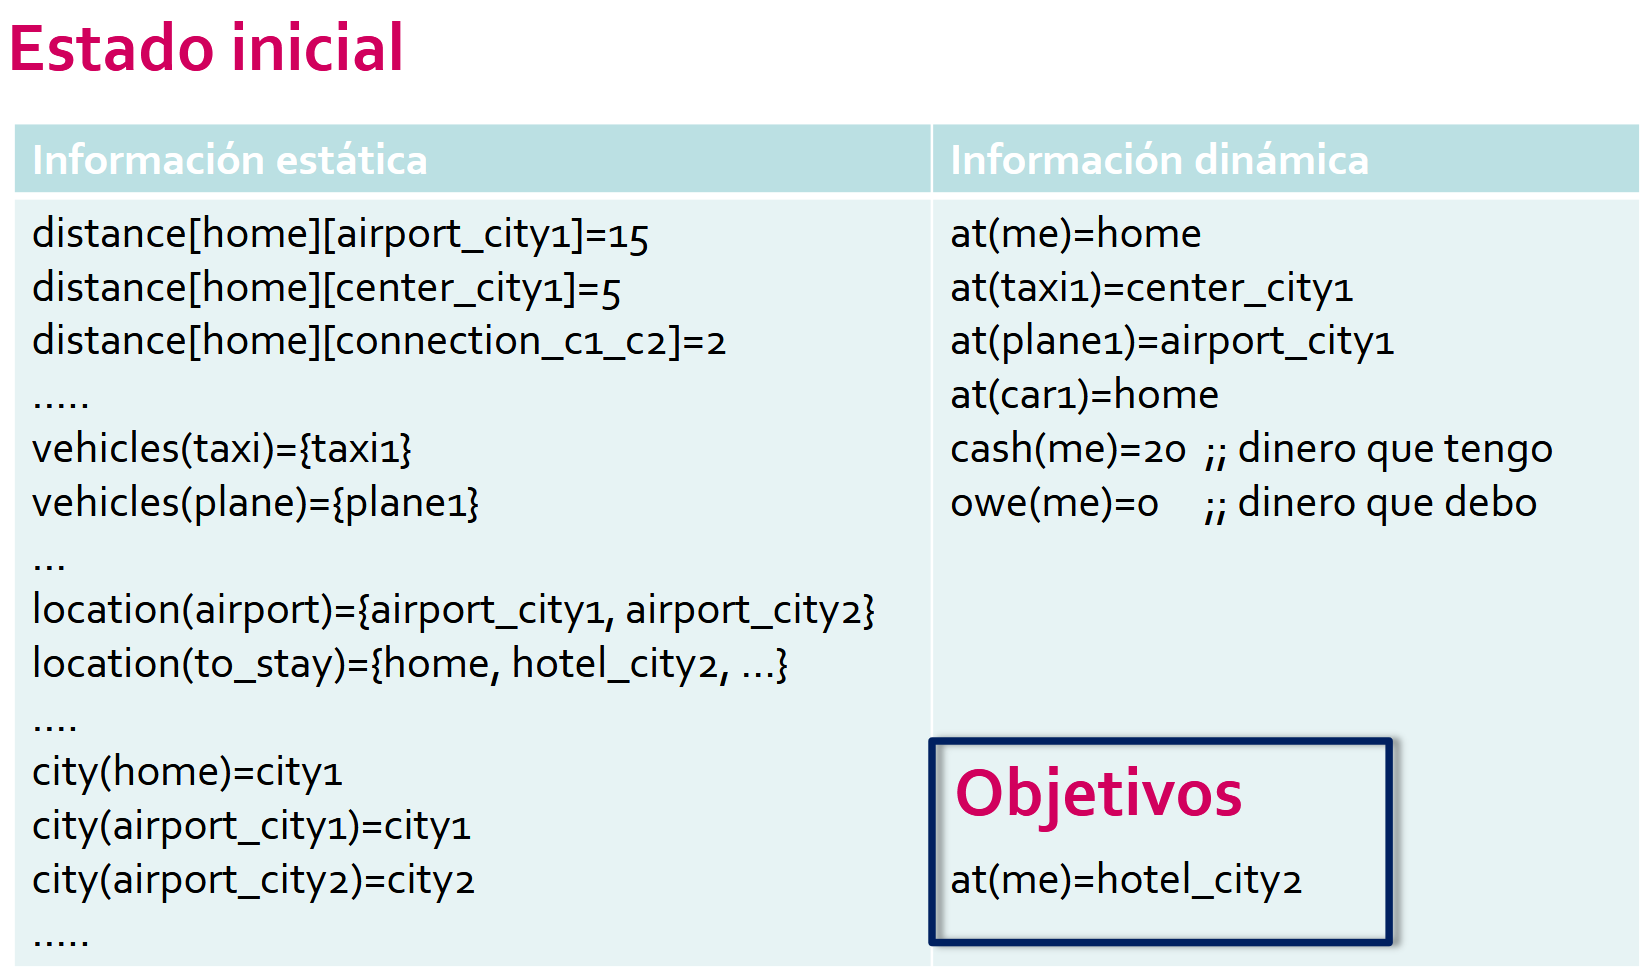
\includegraphics{images/02/estadoinicial.png}
   \caption{Suponen que tengo que viajar desde una ciudad a otra. Esta puede ser una formalización de la planificación.}
   \label{fig:02/estadoinicial}
\end{figure}


\begin{paracol}{2}
   
   Un \textbf{plan} es un conjunto de acciones que se pueden ejecutar en el mundo que Representan los posibles cambios (transiciones) en el entorno. Estas, deben ser independientes de cualquier problema y \ul{se representan con descripciones de condiciones y efectos}:
   \lstinline|a=<Conditions(a), Effects(a)>|
   \begin{itemize}
      \item \lstinline|Conditions(a)|: condiciones que se deben satisfacer en un
      estado para aplicar dicha acción
      \item \lstinline|Effects(a)|: modificaciones del estado actual una vez
      ejecutada la acción
   \end{itemize}

   \switchcolumn

   \begin{figure}[htbp]
      \centering
      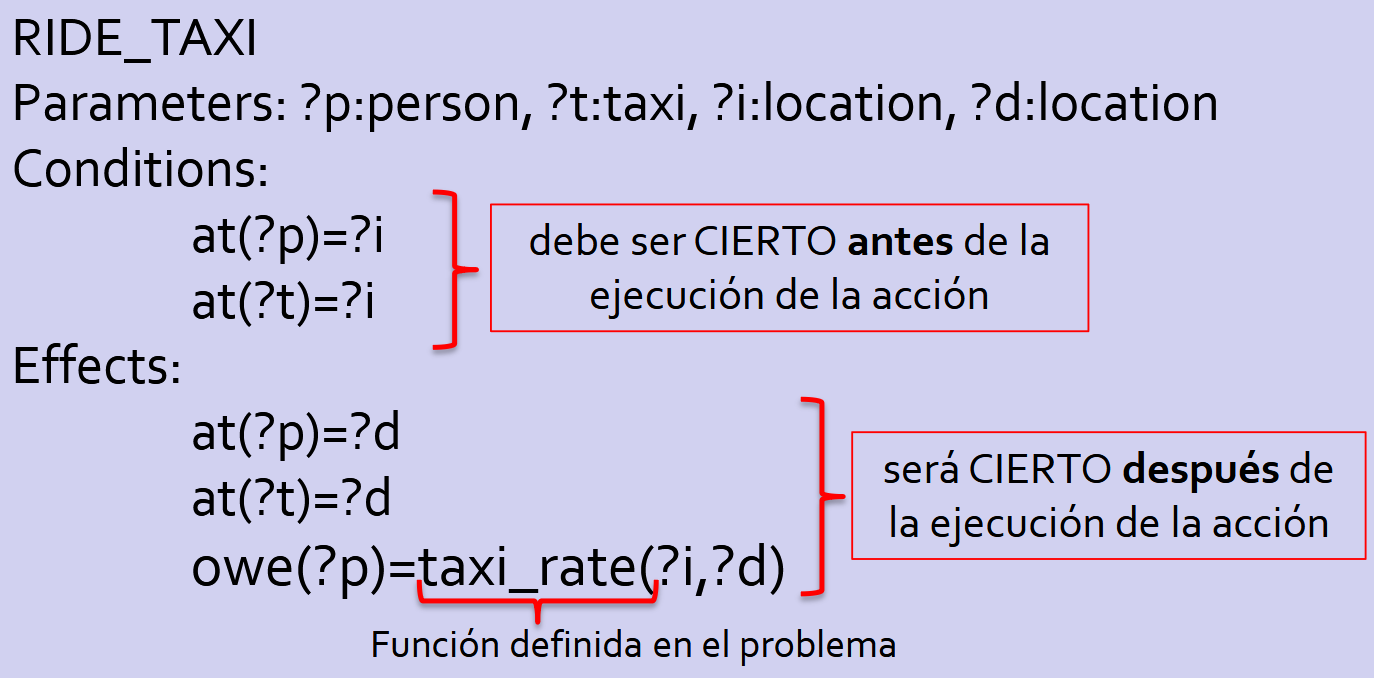
\includegraphics{images/02/condiciones.png}
      \caption{Ejemplo para coger un taxi}
      \label{fig:02/condiciones}
   \end{figure}
\end{paracol}

\begin{definition}[Plan]
   Un plan \lstinline|P| es una secuencia de acciones que transforma el estado
   inicial (\lstinline|I|) en un estado que satisface los objetivos (\lstinline|G|)
\end{definition}

\begin{paracol}{2}
   Un plan puede estar parcial o totalmente ordenado.
   Un enlace causal ($a_i$, $p$, $a_j$ ) determina que la acción ai resuelve la condición $p$ de la acción $a$.
   

   \switchcolumn

   \begin{figure}[htbp]
      \centering
      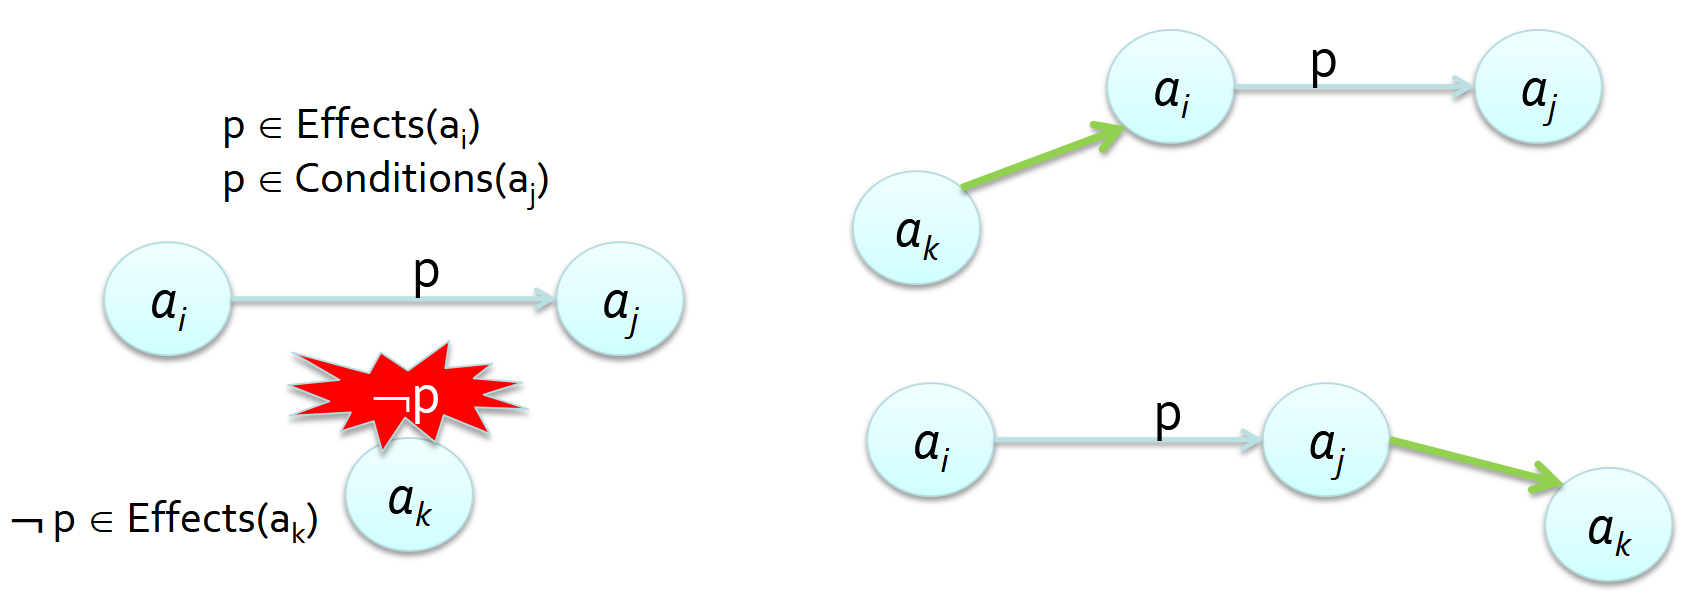
\includegraphics{images/02/planordenado.png}
      \caption{Plan}
      \label{fig:02/planordenado}
   \end{figure}

\end{paracol}

\subsubsection{Modelo ``planificación clásica''}
\begin{itemize}
	\item Determinista
	\item Estático (solo cambia por las acciones)
	\item Completamente observable
	\item Razonamiento temporal y numérico no contemplado
\end{itemize}

Es decir, el resultado de una acción aplicada a un estado
completamente conocido se puede predecir correctamente,
ya que no hay influencias externas que afecten al entorno.Para resolver este problema se utilizan algoritmos de búsqueda.

Esto modelo pero es muy limitado, y sus asuciones necesitan ser relajadas para que sea más realista y aplicable a problemas reales.\\
En primer lugar, las acciones tienen distintas \textbf{duraciones}, usan recursos y tienen \textbf{coste}; además, El mundo \textit{no} es totalmente conocido (existe incertidumbre) y es \textbf{dinámico} (cambia debido a eventos exógenos).


\section{Planificación Jerarquica}


La idea principal de \textbf{HTN} Hierarchical Task Network planning es proceder de una forma más parecida
a como los humanos resolvemos los problemas complejos:
Primero los aspectos generales (tareas) y después los detalles.


\begin{paracol}{2}
   
   Se definen métodos abstractos que se deben descomponer
   para resolver el problema.
   Métodos son los triángulos invertidos en la figura.

   Cada método incluye estos componenetes:
   \begin{itemize}
      \item Nombre
      \item Párametros
      \item Precondiciones
      \item Red de tareas
   \end{itemize}
   \switchcolumn

   \begin{figure}[htbp]
      \centering
      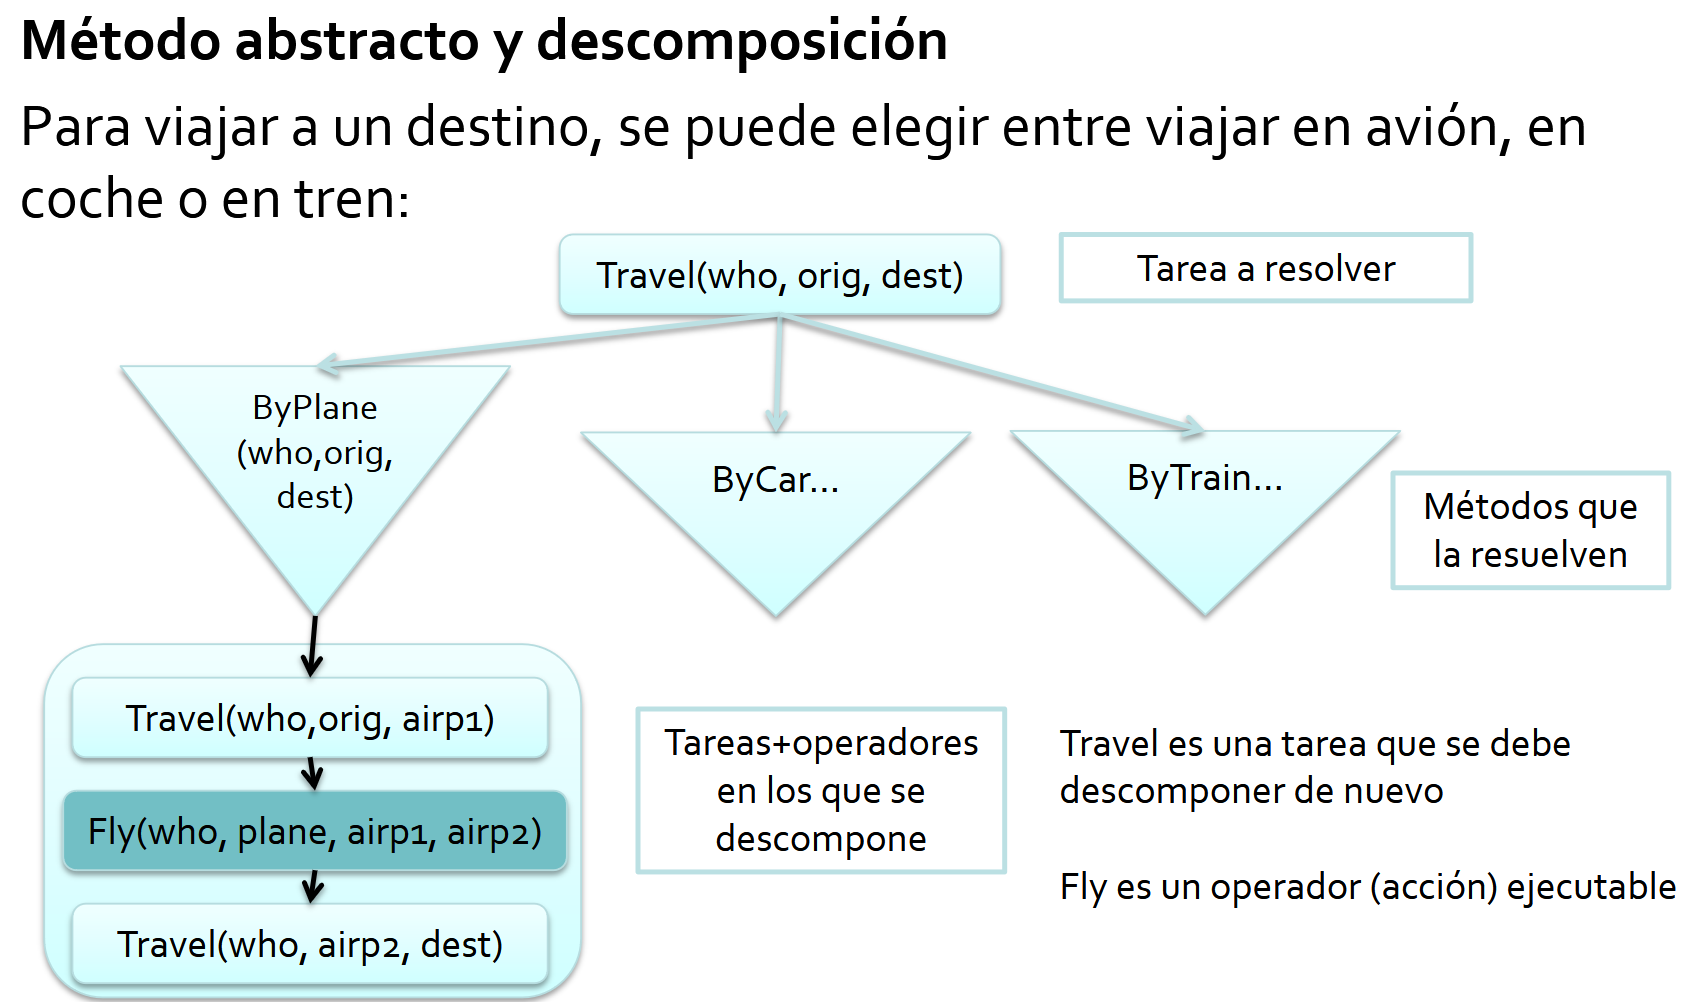
\includegraphics{images/02/htn.png}
      \caption{Método abstracto y decomposición}
      \label{fig:02/htn}
   \end{figure}
\end{paracol}


\begin{paracol}{2}
   Métodos son tareas a descomponer, y los operadores (como \lstinline|Fly|) representan las acciones que se pueden llevar a cabo dentro del
   mundo para poder alcanzar los distintos objetivos (acciones
   ejecutables que producen cambios en el estado del mundo).
   \begin{itemize}
      \item Nombre
      \item Parámetros
      \item Condiciones
      \item Efectos
   \end{itemize}
   
   \switchcolumn

   \begin{figure}[htbp]
      \centering
      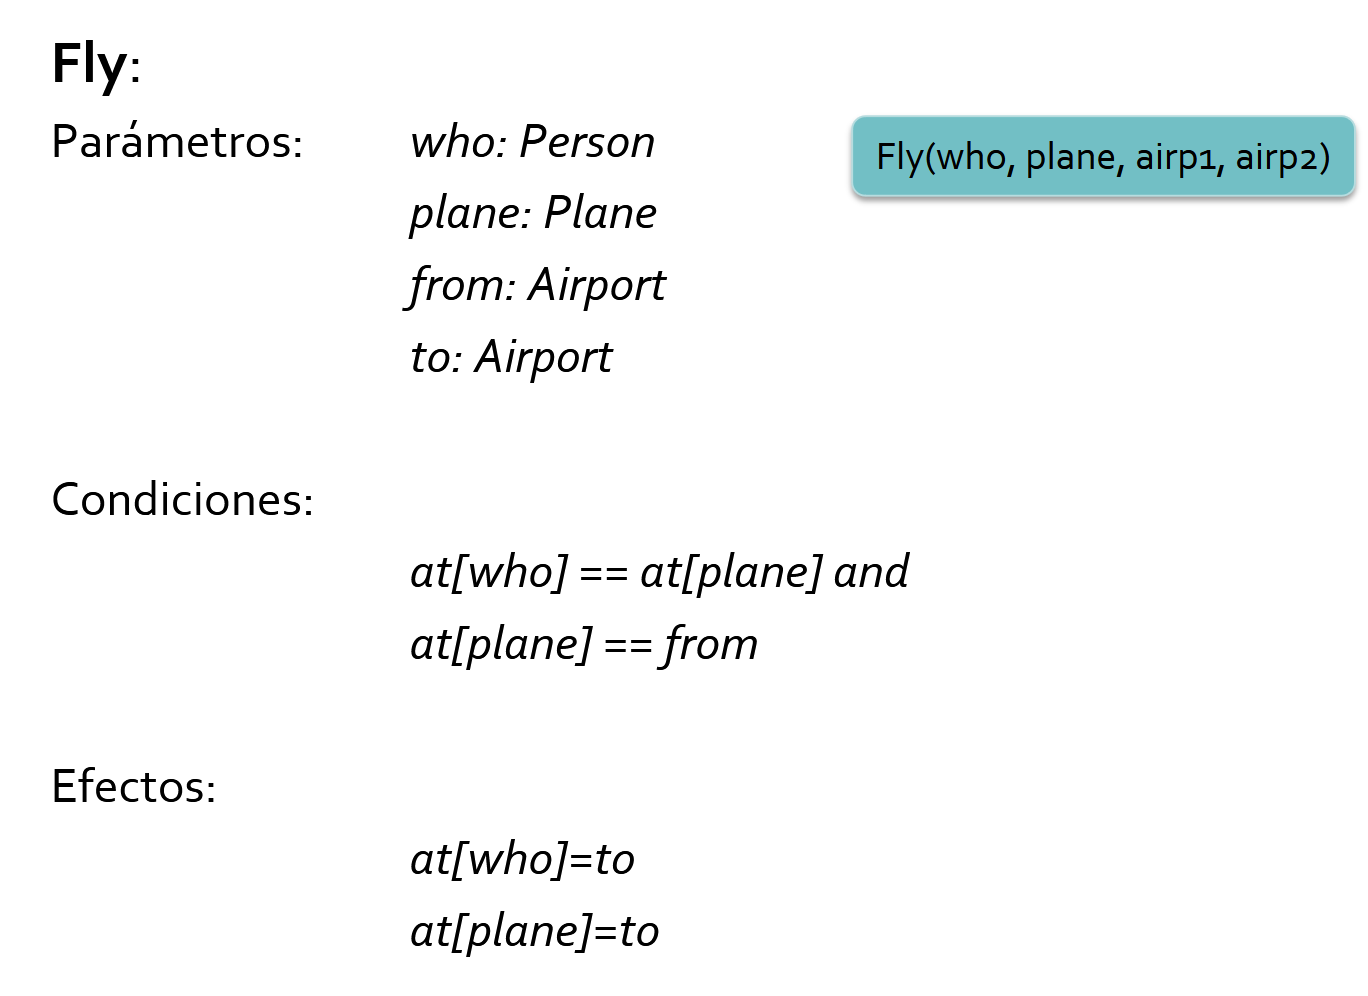
\includegraphics{images/02/accionFly.png}
      \caption{Accion \lstinline|Fly|}
      \label{fig:02/accionFly}
   \end{figure}
\end{paracol}